\begin{figure*}
  \centering
  \setlength\tabcolsep{0pt}
  \renewcommand{\arraystretch}{0}
  \begin{tabular}{lc}
                                                                                                                               &
    \includegraphics[width=0.95\linewidth, trim=0 656 1255 0, clip]{fig/\conerfdirname/novel_view_nosynth/figures.pdf}           \\
    \multirow[t]{-2}{*}{\includegraphics[width=0.032\linewidth, trim=0 -20 0 0, clip]{fig/novel_view_nosynth/left-legend.pdf}} &
    \includegraphics[width=0.95\linewidth, trim=0 0 1255 450, clip]{fig/\conerfdirname/novel_view_nosynth/figures.pdf}           \\
                                                                                                                               &
    \includegraphics[width=0.95\linewidth, trim=1260 656 0 0, clip]{fig/\conerfdirname/novel_view_nosynth/figures.pdf}           \\
    \multirow[t]{-2}{*}{\includegraphics[width=0.032\linewidth, trim=0 -20 0 0, clip]{fig/novel_view_nosynth/left-legend.pdf}} &
    \includegraphics[width=0.95\linewidth, trim=1260 0 0 450, clip]{fig/\conerfdirname/novel_view_nosynth/figures.pdf}
  \end{tabular}
  \renewcommand{\arraystretch}{1}
  % \begin{subfigure}[b]{0.796\linewidth} \centering %
  % 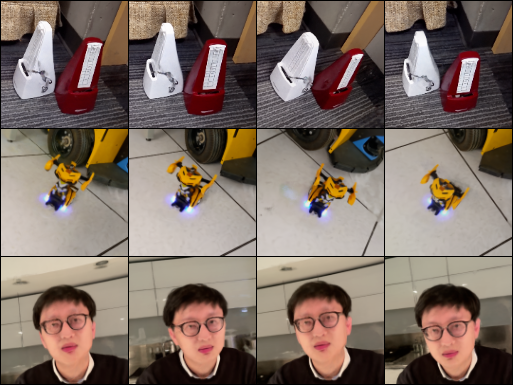
\includegraphics[width=\linewidth]{fig/assets/novel view/view.png}
  % \includegraphics[width=\linewidth]{fig/assets/update-attributes.pdf}
  % \caption{attribute interpolation} \end{subfigure} \hfill{}
  % \begin{subfigure}[b]{0.1925\linewidth} \centering
  % \includegraphics[width=\linewidth]{fig/assets/update-views.pdf}
  % \vspace{-0.22em} \caption{novel view synthesis} \end{subfigure}
  \caption{{\bf Novel view and novel attribute synthesis --}
    We synthesize scenes from a novel view and with a novel attribute
    combination, not seen during training.
    % \ky{
    A naive extension of HyperNeRF, HyperNeRF{+}$\pi$ fails to disentangle
    attributes and results in a modification of the scene irrespectively of
    attribute meaning \eg, opening mouth results in closing eyes at the same
    time.
    % is not what the attributes are describing--- and vice versa. 
    \textbf{Ours}-$\MaskNet$ improves the results, but does not disentangles the attribute space, as successfully done by our complete method. % results in entanglement.
    The differences between these methods can even lead to complete failure
    cases, as shown in the metronome and the toy car case.
  }
  % \cite{park2021hypernerf} with a projection network $\mathcal{A}$ to predict
  % attribute values $\{\attribute_\iAttribute\}$ causes that changes in the
  % output become entangled, \eg, opening the mouth also closes the
  % eyes.%causes closing eyes. }
  \label{fig:conerf-novel_view}
\end{figure*}